\section{PS7: Kronos Log Parsing}\label{sec:ps7}
\graphicspath{{ps7}}
\subsection{Discussion:}\label{sec:ps7:disc}
    We analyze the Kronos Intouch time clock log by using regular expressions to parse the file.
    Also we verify device boot up timing.
    here we take the given device[1-6]*underscore*intouch.log files and give a resultant file which contains the time, date, status and line number of the boot to the .rpt file.

\subsection{Key algorithms, Data structures and OO Designs used in this Assignment:}
    I used the lambda expression for getting the time from first 19 characters i.e substring(0,19).
    I prefer using lambda expression than ordinary method as its more efficient.
    Just utilized the three functions from the regex library to finish my project.
\subsection{Explanation of the code:}
    Firstly, I initialize regular expressions to the starting and ending log entries so it can be used to compare the regex to find.
    if there is a match in every line of the file(.log). I create an -outputfile where the data of the result is stored as filename.log.rpt .There is a use of bool exp to keep tracking of the incomplete booting. I utilize the regex-search function to search a match for the starting regular expression(log.c.166). 
    if there is no incomplete booting, I write the date,time,line number and status of the boot to our -outputfile. The else if condn is used to search the line for finding the match for the ending regular expression. if that is found, The calculation of the duration of the time is begun by using posix. Again I write the line-number, date , time and duration it took for the completion of sequence.

\subsection{What I accomplished :}

I accomplished creating Kronos log Parsing and approach towards regular expression in C++.

\subsection{What I learned :}

I learnt implementing of the regex library <regex> More efficiently.\newline
I have implemented following regex functions into my code. \newline
\begin{itemize}
    \item boost::regex startMessage("( \\(log.c.166\\) server started)");
    \item boost::regex endMessage("(oejs.AbstractConnector:Started SelectChannelConnector)");
    \item regex-search(s, startMessage)
   \item  regex-search(s, endMessage)
\end{itemize}

\subsection{Challenges :}

Implementing a proper format was challenging to me to the output file.

\subsection{Codebase}\label{sec:ps7:code}

\textbf{\colorbox{pink}{Makefile:}} \newline \textbf{This Makefile has lint.}
\lstinputlisting[language=Make]{ps7/Makefile}

\textbf{\colorbox{pink}{main.cpp:}} \newline \textbf{The main file contains all the regex library as well as time library and functions to achieve the \textit{Kronos Log Parsing}}
\lstinputlisting{ps7/main.cpp}


\subsection{Output:}
\begin{figure}[h]
   \centering
    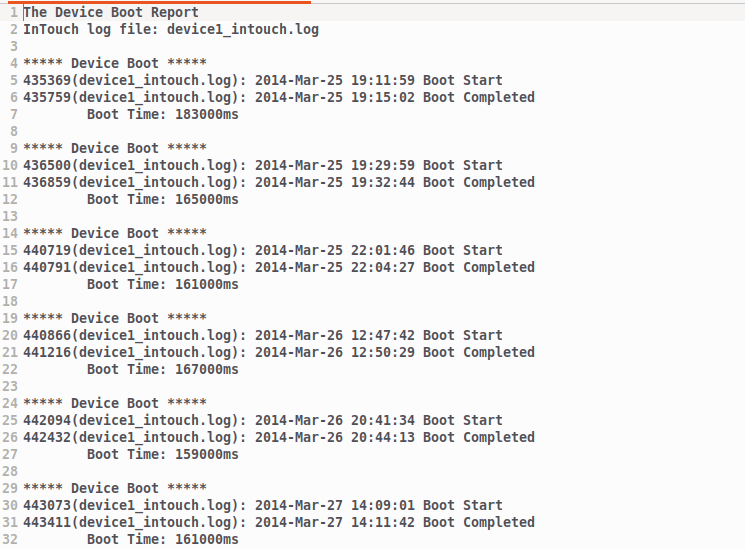
\includegraphics[width=1\textwidth]{ps7/d1.png}
    \caption{device1 output}
    \label{fig:ps7d1}
\end{figure}
\begin{figure}[h]
   \centering
    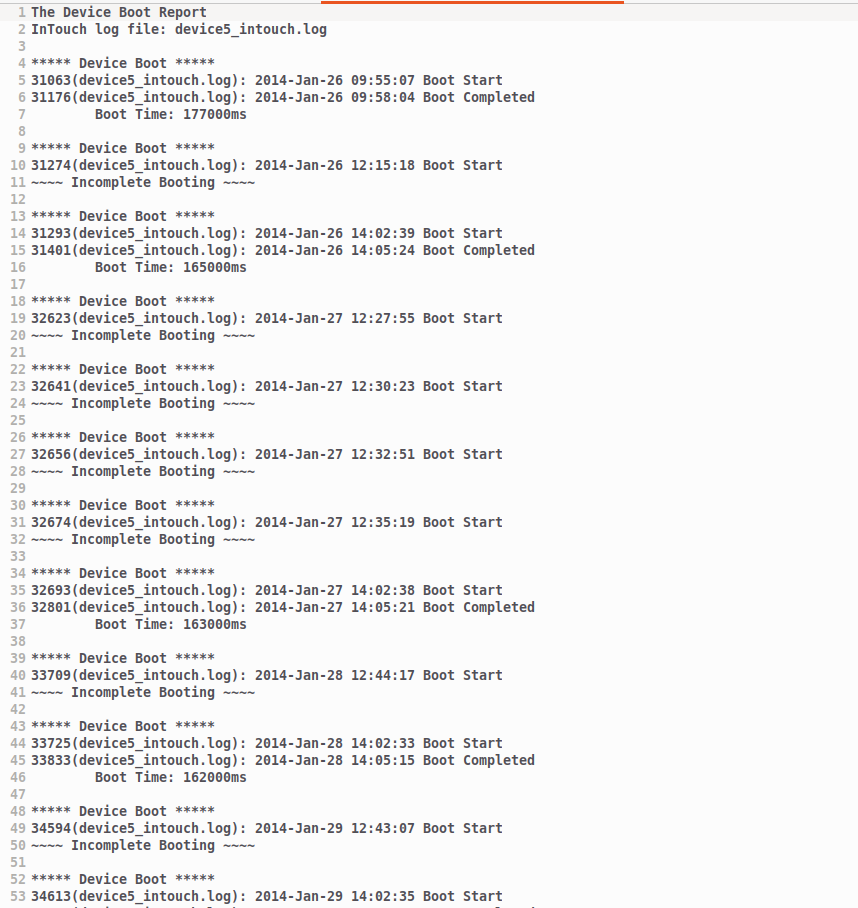
\includegraphics[width=1\textwidth]{ps7/d5.png}
    \caption{device5 output}
    \label{fig:ps7d5}
\end{figure}
\begin{figure}[h]
   \centering
    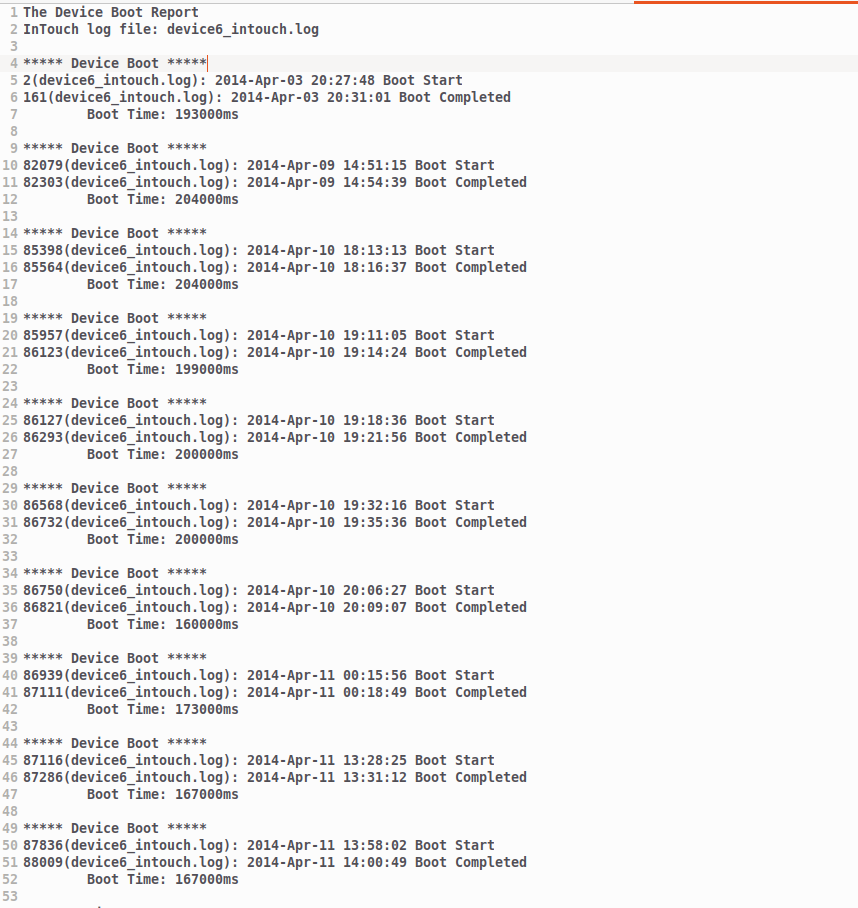
\includegraphics[width=1\textwidth]{ps7/d6.png}
    \caption{device6 output}
    \label{fig:ps7d6}
\end{figure}

\newpage
